\section{Primary Editors}\label{primaryEditors}

\subsection{Score Timeline}\label{scoreTimeline}

Score Timeline

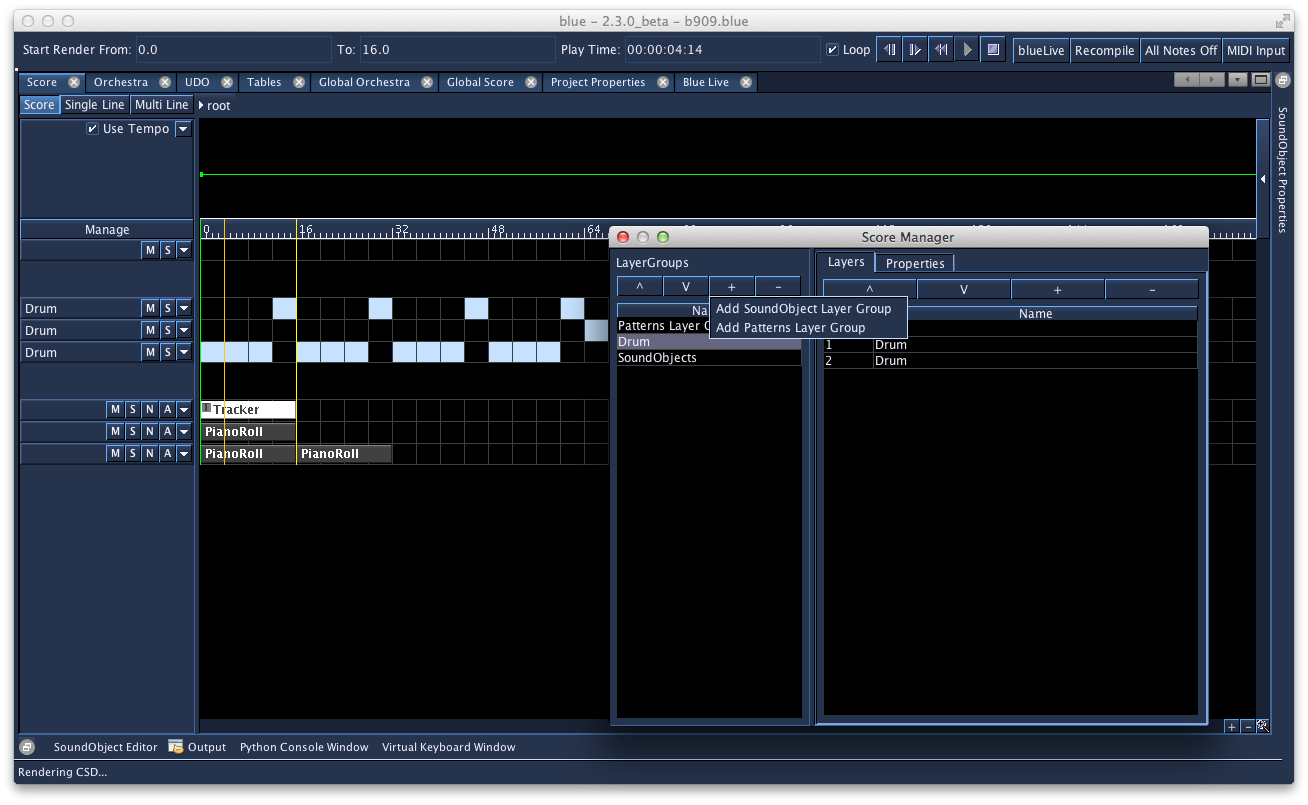
\includegraphics[width=1.00000\textwidth]{images/ScoreTimeline.png}

\subsubsection{Overview}

The Score is the tool in blue for working with musical material in time.
It is a canvas upon which to create and organize musical ideas. The
Score features a modular timeline, where each
\protect\hyperlink{layerGroups}{Layer Group} within the Score is a
module. These modules are a plug-in point that can be extended with
other plug-ins. Each Layer Group in turn may be broken down into layers.

The image above shows a Score with three Layer Groups. The first two are
Patterns LayerGroups, while the last is a SoundObject Layer Group. Also
shown is the ScoreManager dialog (accessible from the Manage button on
the left part of the Score).

\hypertarget{layerGroups}{\subsubsection{Layer Groups}\label{layerGroups}}

A Score is divided into Layer Groups. Each Layer Group has a
user-interface for the main timeline area, as well as a header interface
that shows on the left-hand side. The header area usually shows
meta-information and controls for each of the Layer Group's layers, such
as layer name, muting, soloing, and other features.

By using the Score Manager Dialog, you can add as many Layer Groups as
you like, as well as many layers to each group as you like. You can also
push up and down Layer Groups to reorganize them. The same
add/remove/push up/push down actions are also available for Layers
within a Layer Group.

\begin{quote}
\textbf{Note}

Add/Remove/Push Up/Push Down for layers is also available while working
in the main score area by right-clicking the Layer panels on the right
and selecting the options from the popup menu.
\end{quote}

Also, all LayerGroups support having
\protect\hyperlink{noteProcessors}{NoteProcessors} used with them. Using
a NoteProcessor on a LayerGroup will affect all notes generated within
that LayerGroup. Editing the LayerGroup's NoteProcessors can be done by
right clicking on the root Score node in the
\protect\hyperlink{scoreBar}{Score Bar}, described below.

Regarding the design, a Layer Group is primarily responsible for
generating Csound Score notes. However, they are also able to generate
tables, instruments, and anything else that is usable in Csound. It is
up to the developer to choose what features the Layer Group will use.

SoundObject Layer Groups are one of the primary Layer Group types. They
support the SoundObject system in blue for scoring them in time on the
timeline. They also are the canvas on which
\protect\hyperlink{parameterAutomation}{automations} are drawn.

SoundObject Layer Groups are divided into SoundLayers. Each SoundLayer
can contain SoundObjects of any type as well as have automations
assigned to the layer. Unlike MIDI-based studio software, where layers
are bound to a single instrument or channel in a mixer, blue's
SoundLayers are free to hold SoundObjects that generate any data for any
instrument. This design choice allows freedoms for you to design your
project as you wish, though at the expense of being able to implement
some things which may be commonly found in MIDI-based studio software.

To use the SoundObject system, first create a SoundObject Layer Group
using the Score Manager Dialog. (By default, new projects in blue start
with a single SoundObject Layer Group.) Next, add as many layers as you
would like to the LayerGroup. You can then edit the names of the layers
using the ScoreManager Dialog, or back in the main Score area by
double-clicking the area on the left of the Layer's panel on the left.

On the timeline, rt-clicking on any soundLayer will show menu options
for adding different types of SoundObjects, pasting a SoundObject from
the buffer if any SoundObjects in the buffer are available, as well as
other commands. (Copying and pasting of SoundObjects can also be done
using ctrl-c and ctrl-click on a layer.)

Once you have SoundObjects on the timeline, you can click on them to
select it, or click in an empty area and drag to show a selection
rectangle. You can also add and remove SoundObjects to/from the
selectionn by holding shift when clicking.

Once selected, you can move selected SoundObjects by pressing the mouse
down on one of the selected SoundObjects, then drag to move them in time
as well as up and down layers. If you press shift down when you click,
once you drag you will create clones of the original material and move
them in time. If you move the mouse to the right-side of a SoundObject,
the cursor will change to a resize cursor, and clicking and dragging
will allow you to change the duration of the SoundObject. (Note you can
only resize one SoundObject at a time.)

If you have a single SoundObject selected, you can edit the properties
of the SoundObject by using the SoundObject Property Window. This window
can be opened from the menu "Windows -\textgreater{} Sound Object
Properties" or by using the shortcut "F3". From this window you can
change the name of the SoundObject, its start time and subjective
duration, as well as add and remove NoteProcessors (if the SoundObject
supports it).

To edit a SoundObject, select a single SoundObject and open the
SoundObject Editor window. You can also double-click a SoundObject,
which will set the editor for the SoundObject in the Editor window as
well as focus the SoundObject Editor window. (If the Editor window is
docked, double-clicking the SoundObject will cause the editor to show
the docked window.)

Patterns Layer Groups are based upon the same SoundObject system as the
SoundObject Layer Groups, but presents a different way to working with
these objects. At a high-level, each Pattern layer has one SoundObject
assigned to it. The SoundObject is the source score material for a
Pattern Layer. Selecting boxes in the grid that shows for the Patter
Layer determines where that score material will be used to generate
notes. For music projects that rely on patterns and regular metered
time, using the Pattern Layer Groups can be more efficient for creating
a piece than using SoundObject Layer Groups.

The grid of time for Pattern Layers is currently hardcoded to repeat
every four beats, or one measure at 4/4 time. However, a SoundObject is
not constrained to generate score for only one measure. For example, you
can create a PianoRoll that has a time behavior of "None", and have it
last sixteen beats (four measures). Everywhere that the pattern grid is
selected for the Pattern Layer that uses that SoundObject will then
create that sixteen beat score and start it at the time of the grid box.

Patterns Layer Menu Options

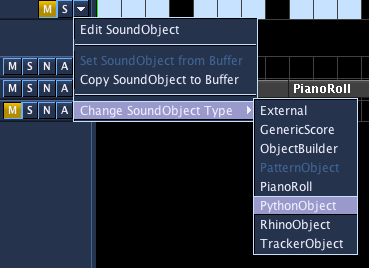
\includegraphics{images/patternLayerMenu.png}

By default, new Pattern Layers will use a GenericScore SoundObject that
is set to a duration of four beats, and use a time behavior of "None".
This means that the score will generate "as-is". In the layer's popup
menu options, you can replace the SoundObject that is being used for the
layer with one from the SoundObject buffer (i.e. copied from blueLive or
from a SoundObject Layer). Also, you can switch to a different type of
SoundObject using the menu.

SoundObjects will generate accordingly to the values set in the
SoundObject Properties dialog, with the exception of the start time.
Blue will reassign the start time to 0 when it generates the notes for
the layer. On the whole this behavior will not affect most users, but is
worth noting.

To edit the SoundObject for a Pattern Layer, you can either use the
popup menu option for "Edit SoundObject", or you can also click the
layer panel on the left. A single click will bring up the SoundObject
editor.

To edit the layer's patterns, click on a grid box to toggle between on
and off for that box. You can also press down and drag along to set
multiple boxes. The value that is set for the multiple boxes will depend
on the action of the first box selected. For example, if the first box
when the initial mouse down is on, the mouse down will turn it off, and
dragging will turn off all boxes that the mouse extends through.

Audio Layer Groups provide standard Digital Audio Workstation (DAW)
functionality. Users can use Audio Layers to drag-and-drop Audio files
onto the timeline. Each Audio Layer maps to a channel in Blue's mixer,
where effects can be added for the audio layer. Automation for effect
parameters is available on the audio layer.

To use the Audio layers, first create an Audio Layer Group using the
Score Manager Dialog. Next, add as many layers as you would like to the
LayerGroup. You can then edit the names of the layers using the
ScoreManager Dialog, or back in the main Score area by double-clicking
the area on the left of the Layer's panel on the left. The name of the
Audio layer will also show under its corresponding mixer channel.

To add Audio files to a layer, you can either drag and drop a file from
the operating system's file mananger, or you can use the Blue File
Manager to locate a file, then drag and drop it to an Audio layer.

Once an audio clip is on the timeline, you can modify its properties in
a few ways. First, you can click and drag it to move it in time. If you
click and drag from the left hand side, you will alter both the audio
clip's start time, as well as the audio clip's file start time. For
example, if a clip was added that started at time 0.0 and had an audio
file start of 0.0, if you drag from the left hand side to time 3.0, both
the start of the clip and audio file start will be set to 3.0. This
means that 3.0 beats into the project, the audio clip will start
rendering from 3.0 seconds into the file. If you drag from the right
hand side, it will alter the duration of the audio clip. If you hold
down alt+shift, then press within an AudioClip, you will split the
AudioClip into parts. If you hold down the alt key, then press and drag
the mouse, you can alter just the file start time.

If you have a single Audio clip selected, you can edit the properties of
the clip by using the ScoreObject Property Window. This window can be
opened from the menu "Windows -\textgreater{} Sound Object Properties"
or by using the shortcut "F3".

Additionally, if a single Audio clip is selected, additional properties
are available to edit using the ScoreObject Editor window. You can also
double-click an Audio clip, which will set the editor for the clip in
the Editor window as well as focus the ScoreObject Editor window. (If
the Editor window is docked, double-clicking the clip will cause the
editor to show the docked window.)

Audio clips support fades. Like Ardour, upon which much of the audio
layer system is based, all fades are crossfades. Clips will crossfade
with signals that are already in the bus, with the first clip
crossfading with silence. Fade types and durations may be set within the
clip's editor panel. The clip duration may be visually modified by
mousing over the clip, pressing with the mouse on either the fade-in or
fade-out handle that appears after mousing over the clip, then dragging
and releasing to update the fade's duration. The fade type may also be
modified by right clicking within a fade area and choosing the fade type
using the popup menu.

For more information about Fades, please see Ardour's manual entry on
\href{http://manual.ardour.org/editing-and-arranging/create-region-fades-and-crossfades/}{Region
Fades and Crossfades}.

\subsubsection{User-Interface Walkthrough}

The play bar at the top has:

\begin{itemize}
\tightlist
\item
  time to start playing from
\item
  what time to play to (if the render end time is set)
\item
  the current play time
\item
  Loop checkbox to have render looping from render start time to render
  end time
\item
  Forward/Back buttons for jumping between markers
\item
  Back button to start from beginning of Score
\item
  Play/Stop buttons to start/stop rendering
\item
  BlueLive buttons:

  \begin{itemize}
  \tightlist
  \item
    blueLive toggle button to turn on/off blueLive
  \item
    Recompile button that will stop the current blueLive run, recompile
    the project, and start blueLive again
  \item
    All Notes Off Button to turn off any hanging notes in a blueLive run
  \item
    MIDI Input toggle button enabled/disables blue MIDI input into
    blueLive
  \end{itemize}
\end{itemize}

the poly object bar (shown above with only one polyObject, "root") shows
what polyObject you are currently editting. if you were to add a
polyObject named "phrase 1" to the main timeline shown above, then
double click that polyObject to edit it, the polyObject bar would have
two buttons on it, one for "root", and one for "phrase 1". you would
then be editting "phrase 1"'s timeline. by clicking on the "root" button
of the timeline, you would then return out of the polyObject's timeline
and back in the root's timeline.

Below the polyObject bar on the left, you will see the soundLayer
edittor. here you can change the name of the soundLayer, as well as mute
the layer (all soundObject's on muted layers will not be used to
generate notes when creating .CSD files).

on the bottom of the soundLayer edittor are four buttons, "\^{}", "V",
"+", and "-". "\^{}" and "V" will push up or push down soundLayers.
(HINT: You can move multiple soundLayers by clicking on one soundLayer,
then holding down shift and clicking on the last of the soundLayers you
want to move, then using the "\^{}" and "V" buttons.) the "+" will add a
soundLayer after the currently selected soundLayer. if no soundLayers
are selected, then it will add one to the end of the list. the "-"
button will remove any selected soundLayers. it should ask for a
confirmation before removing any layers.

Below the polyObject bar on the right is the main time line. it shows
the time line for the currently editted polyObject. The +/- buttons next
to the scrollbars are used to zoom in on the time line, and those
settings will be maintained between work sessions.

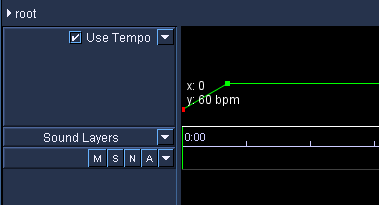
\includegraphics{images/tempo_editor.png}

The tempo editor is an optional use feature that allows editing of
overall tempo for a project using a line editor. This feature starts off
as disabled and closed. When in this state, whatever tempo values are
saved will show as dark gray line that is uneditable. To enable the use
of the tempo editor, select the checkbox marked "Use Tempo". Selecting
this will redraw the tempo line in green. To open up the tempo editor
for a larger view and for editing, select the down arrow button next to
the "Use Tempo" checkbox.

Like other line editor objects in blue, left-clicking on an area where
there is no point will insert a new point, while hovering over an
existing point and pressing down, then dragging will allow moving of
that point. Right-clicking a point will delete a point.

If right-clicking the tempo editor when not on a point, the following
popup menu will appear:

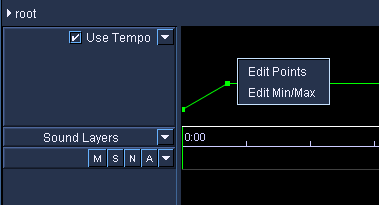
\includegraphics{images/tempo_editor_popup.png}

The first option will allow editing of the values of the points entered
into the line editor by use of a table with two columns: the first
column being the beat on which the tempo change occurs and the right
column being the tempo value that it should have. One may find using the
table editor easier to use to fine-tune values.

The second option will allow changing the boundary min and max tempo
values for the line editor, as well as the option for what to do for
points that fall outside of the new range. The options here are
"Truncate" which will set any points' values that lie outside the new
range to the closest boundary value, or "Scale" which will take all
point values from the old range and scale them to the new range.

Use of the tempo editor is completely optional and users familiar with
Csound's t-statement for controlling global tempo may opt to disable
using blue's tempo editor and to use a t-statement in the global orc
section of the globals tab. Also, older blue projects that existed from
before blue's tempo editor was developed can count on their projects
loading and running correctly even if opened with versions of blue that
do have a tempo editor, due to blue's default to disable the blue tempo
editor. Regardless of which tempo system is chosen by the user, one
should be careful not to use both at the same time as this will cause
two t-statements to exist in the generated CSD (the hand-entered one and
the one generated by blue), causing unexpected performance results.

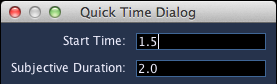
\includegraphics{images/quickTimeDialog.png}

While in the main timeline area, pressing ctrl-t when a soundObject is
selected will bring up the quick time dialog. Here you can edit the
start time and duration of the currently selected soundObject. When the
dialog is first popped up the start time field is automatically focused
for editing. You can press tab to switch between the two fields.
Pressing enter will update the properties. Pressing escape, closing the
dialog, or clicking anywhere outside of the dialog will cancel any
changes and close the dialog.

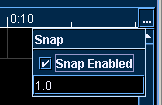
\includegraphics{images/snap.png}

In the upper right of the Score window is an arrow button; pressing this
reveals the time properties for the Score. The two options here are Snap
and Time Display. Snap provides a grid by which to line up your
SoundObjects. Snap is measured in beats. Time Display allows setting how
the time bar shows numbers, i.e. every 4 beats, rendered as a number or
as a time value.

\begin{longtable}[]{@{}ll@{}}
\caption{Shortcuts for the Timeline}\tabularnewline
\toprule
Shortcuts & Description\tabularnewline
\midrule
\endfirsthead
\toprule
Shortcuts & Description\tabularnewline
\midrule
\endhead
ctrl-c & copy selected soundObject(s)\tabularnewline
ctrl-x & cut selected soundObject(s)\tabularnewline
ctrl-click & paste soundObject(s) from buffer where
clicked\tabularnewline
shift-click & paste soundObject(s) from buffer as a PolyObject where
clicked\tabularnewline
shift-click & when selecting soundObjects, adds soundObject to selected
if not currently selected and vice-versa\tabularnewline
double-click & if selecting on timeline, select all soundObjects on
layer where mouse clicked\tabularnewline
ctrl-d & duplicate selected SoundObjects and place immediately after the
originals\tabularnewline
ctrl-r & repeat selected SoundObjects by copying and placing one after
the other n number of times where n is a number value entered by the
user (user is prompted with a dialog to enter number of times to
repeat)\tabularnewline
ctrl-drag & if ctrl is held down when drag is initiated of selected
SoundObjects, a copy of the originals is made and left at their original
times\tabularnewline
ctrl-t & show quick time dialog\tabularnewline
alt-1 & switch to Score mode\tabularnewline
alt-2 & switch to Single Line mode\tabularnewline
alt-3 & switch to Multi Line mode\tabularnewline
\bottomrule
\end{longtable}

\subsection{Orchestra Manager}\label{orchestraManager}

Orchestra Manager

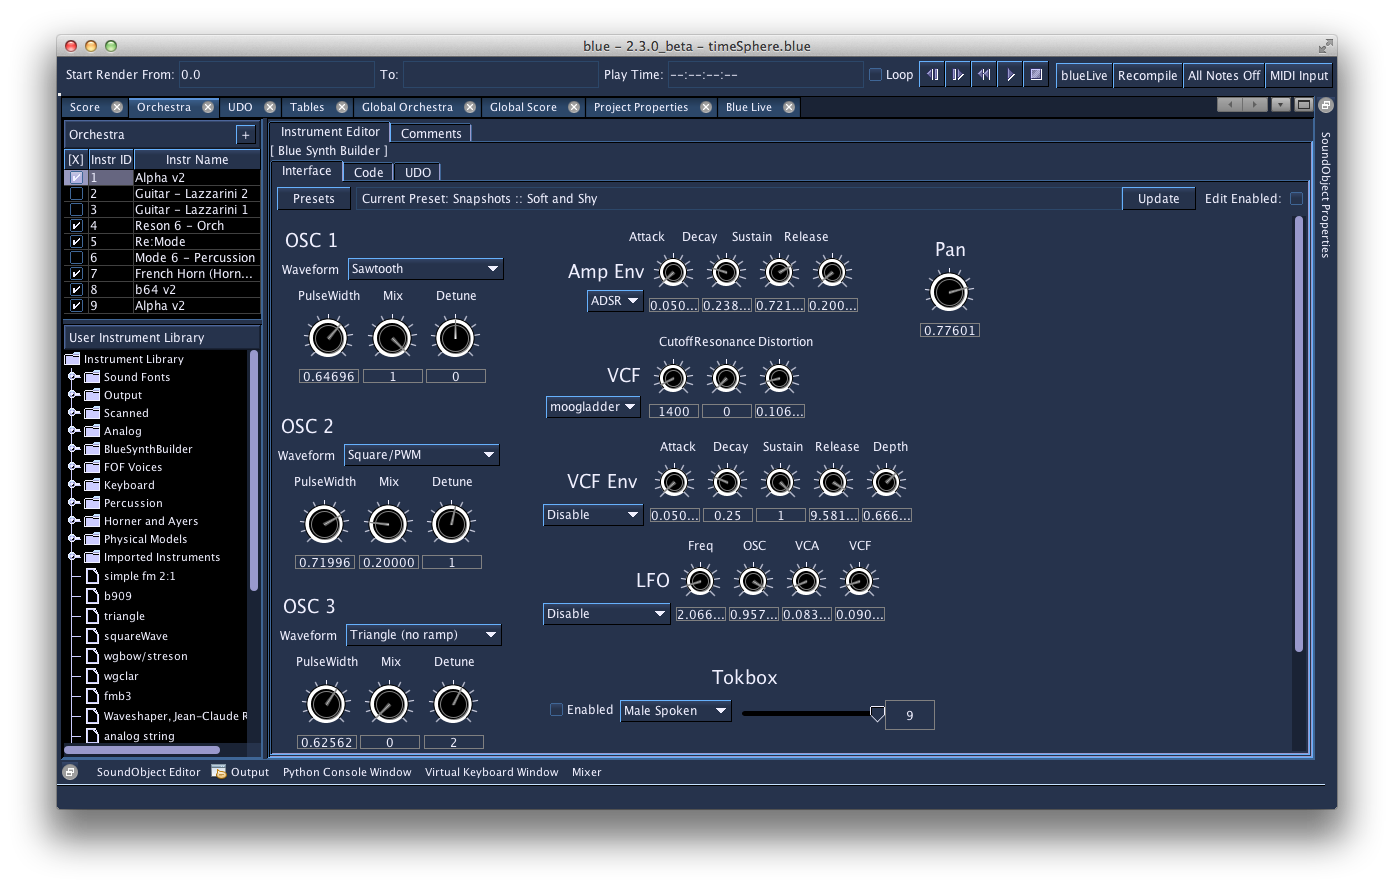
\includegraphics[width=1.00000\textwidth]{images/orchestra.png}

The Orchestra Manager is where the user organizes and edits the
orchestra for the project as well as their user Instrument Library.

In the User Instrument Library (the tree pictured on the left), you can
create instruments as well as categorize them into groups. Most actions
in this editor are accessible by right clicking with the mouse to access
popup menus. (keyboard shortcuts of ctrl-x, ctrl-c, and ctrl-v work for
cutting, copying, and pasting nodes of the tree). To edit the name of
Instruments or Groups, double click the name in the tree or hilight the
node and press F2. This library of instruments is available across
projects and is useful for building up and organizing a personal
instrument library.

To copy instruments into the library from the project's Orchestra, you
can drag and drop the instrument on the library tree to make a copy of
the instrument. To copy an instrument from the Library to the project's
orchestra, you can similarly drag and drop an instrument from the
Library to the Orchestra. You may also use cut/copy/paste to move
instrument from one to the other.

The Orchestra panel (located in the top left of the picture) is where
you will place your instruments to be used for your project. The "+"
button allows you to create new instruments from one of the available
Blue instrument types. You can also right-click on the Orchestra to show
options for copying/pasting. Once instruments are in the Orchestra, you
can edit what their instrument ID's: these may be either numbers or
strings (i.e. 3 for "instr 3", violin for "instr violin"). Selecting an
instrument will show its editor in the Instrument editor section on the
right.

On the right hand side of the Orchestra Manager is the area for editing
instruments. To make more space available for editing an instrument, you
can drag the split pane splitter to the left, or double-click the
splitter to have it collapse to the left-hand side. Each blue
instrument-type has its own editor. Note: if you are editing and
instrument from the Library, blue will show a green border with the
title "Editing Library Instrument" to help notify you what instrument
you are editing.

For projects before 0.94.0, imported projects will have their
instruments largely setup in the same way as they were before.

For projects that were in the 0.94.0 beta series, per-project Instrument
Libraries will be removed. An option to import the instrument library
will be presented to the user and if the user agrees, a folder entitled
"Imported from Project" will be added to the root of the user's
InstrumentLibrary. On the whole, it is recommended to import the
library, review the instruments, and simply remove what is not
necessary. Deleting the imported library is as simple as deleting the
folder for the imported group. Instruments in these project's
Arrangements will be modified to hold copies of the instruments from the
library as opposed to being references to instrument in the library.
(Previously, if two instruments in the Arrangement pointed to the same
instrument in the per-project InstrumentLibrary, changes to the
instrument in the library would affect all instruments in the Arrangment
that pointed to it. Now, only copies are made and no references are
used.)

\subsection{User-Defined Opcodes Manager}\label{udoManager}

User-Defined Opcodes Manager

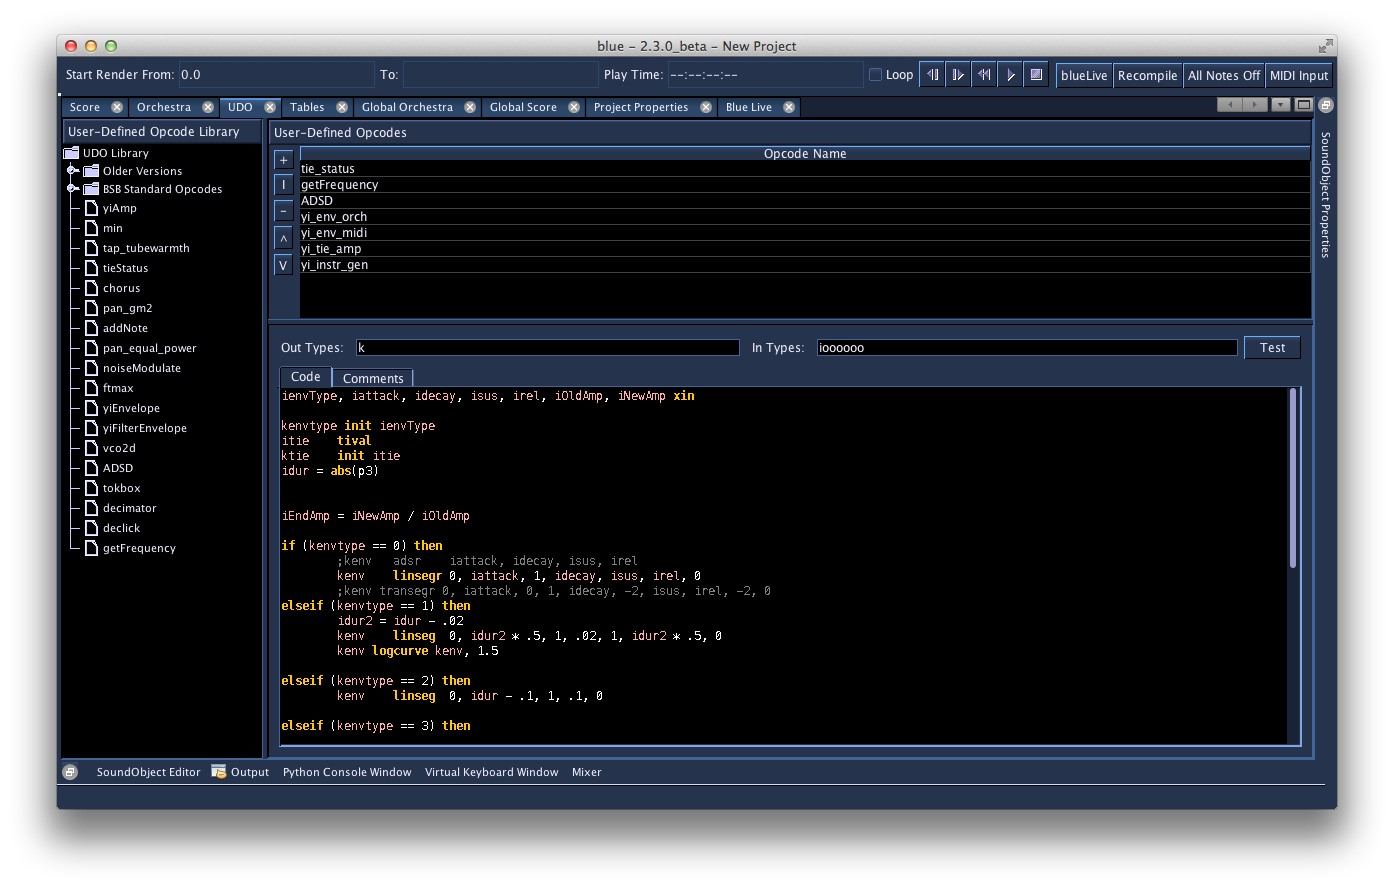
\includegraphics[width=1.00000\textwidth]{images/udoWindow.png}

The User-Defined Opcodes Manager contains three main parts:

\begin{itemize}
\tightlist
\item
  Program-wide User-Defined Opcode Library
\item
  UDO list for Project-wide UDO's
\item
  UDO Editor
\end{itemize}

The program-wide UDO library is where you can manage your entire library
of UDO's. Right-clicking on the tree allows adding and removing groups,
as well as adding and removing UDO's. You can also drag UDO's into the
library from the project-wide UDO list, or paste them using the popup
menu. Clicking on a UDO in the library will populate the UDO Editor, and
a green border will be shown to highlight that you are editing the
library copy of the UDO.

The project-wide UDO list contains what UDO's are available for your
project. Since UDO's can be embedded into Blue instruments, it is
usually better to do so so that an instrument is encapsulated and
copying the instrument will include all of its UDO's it depends on.
However, using the project-wide UDO list can be useful when creating a
new project and multiple new instrument designs might be using a
developing UDO.

UDO's can be created in the project-wide list by using the "+" button,
and removed by using the "-" button to the left the table on top. UDO's
can also be dragged into this list from the library. You can also drag
in a folder of UDO's from the library into this list, or copy/paste them
using the popup menu. Dragging a folder is useful if you have a set of
UDO's you commonly use in all of your instrument designs.

As UDO's may depend on other UDO's, the order in which they are
generated can be significant. The UDO's in the table are generated from
top-down. To shift the order of the opcodes up and down, select an
opcode in the table and use the "\^{}" and "V" buttons to push up and
push down.

To edit the UDO, select one from the table. After selecting a UDO, the
UDO Editor will be populated with that UDO. This time, no green border
will show, as that is only done when a Library UDO is being edited.

For UDO's, you will need the name of the UDO, the intypes and outtypes,
and the body of the code itself. For the body of the code, you will not
need anything from the "opcode" line that normally starts a UDO
definition (i.e. "opcode myOpcode, a, ak"), as those should be in the
text fields for Opcode Name, In Types, and Out Types, and you will not
need an "endop", as blue will add that itself.

User-Defined Opcode Repository Browser

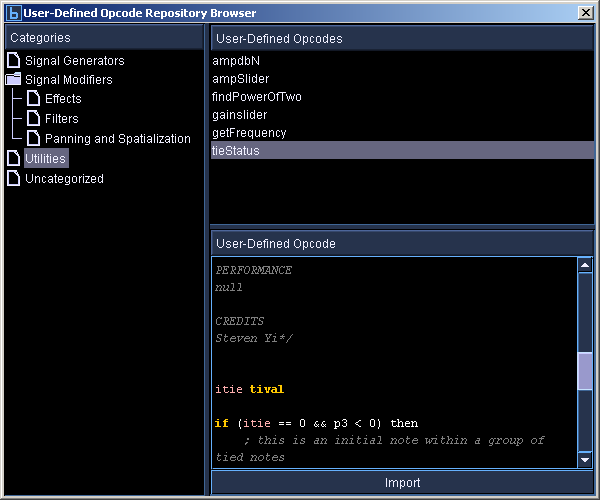
\includegraphics{images/udoDB.png}

Using the "I" Button will open up the UDO Repository browser. The
browser shows the available UDO's in the repository on Csounds.com and
allows for importing from the repository straight into your project.

\subsection{Project Properties}\label{projectProperties}

Project Properties

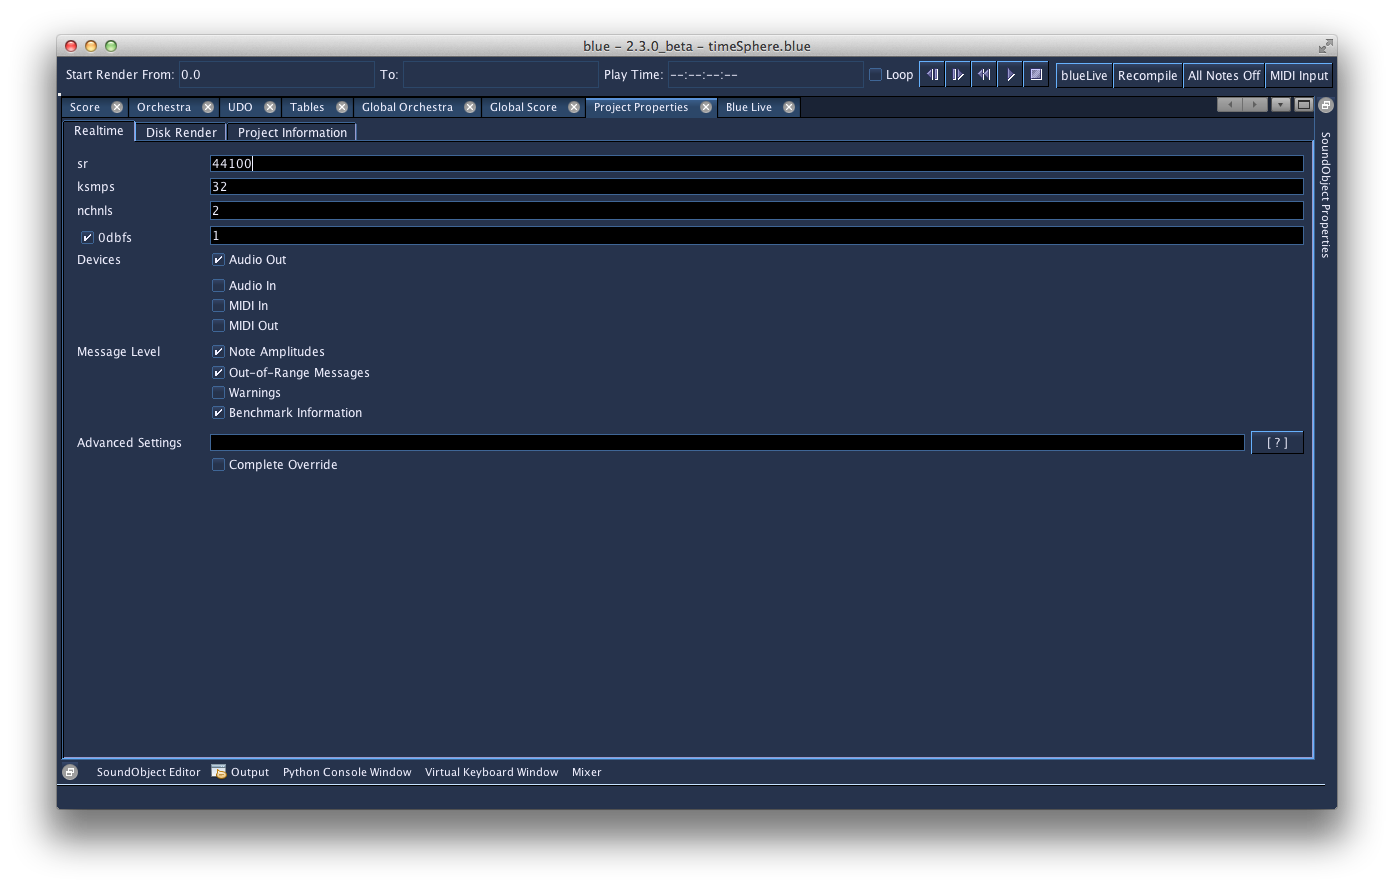
\includegraphics[width=1.00000\textwidth]{images/projectProperties.png}

\begin{description}
\item[sr]
sr to use when rendering in real-time. Value defaults to value set in
Program Options.
\item[ksmps]
ksmps to use when rendering in real-time. Value defaults to value set in
Program Options.
\item[nchnls]
nchnls to use when rendering in real-time. Value defaults to value set
in Program Options.
\item[0dbfs]
The checkbox sets whether 0dbfs is used at all in the project. If
enabled, the value will be assigned to the value in the textfield. The
default for the value is set ing Program Options, as well as if 0dbfs is
enabled by default or not.
\item[Devices]
Devices to use when rendering in real-time (Audio In/Out, MIDI In/Out).
The value of the device is dependent on the values set on the Program
Options. By delegating the value to use to what is set on the Program
Options, the project does not have to store settings which are hardware
dependent, so projects can be easily moved from one computer to the
next.

For example, if your project is set to use "Audio Out", one system may
use a value of "-+rtaudio=alsa -o dac:hw:0,0" while another system may
use a value of "-+rtaudio=winmme -o dac2". The project only needs to be
set to use "Audio Out" and when the project goes to render, the settings
set for that system's audio out will be used.
\item[Message Level]
Enables what kind of messages Csound should report. The values default
to what is set in Program Options.
\item[Advanced Settings]
Extra flags to append to the commandline that might not be covered by
options in the UI. Pressing the {[}?{]} button will open the
documentation for the Csound command flags (Csound Documentation Root
but be set for this to work).

If "Complete Override" is enabled, the value given in the "Advanced
Settings" textbox will be used as given and no other values set from the
UI will be used. Projects prior to 0.106.0 will have their commandline
settings copied to here and the "Complete Override" section will be
enabled. When this setting is enabled, the commandline should set the
call to the Csound executable to use and the flags to use but with the
name of the CSD left out as it will automatically be appended to by
blue. An example of a commandline to use here with "Complete Override"
is:

\begin{verbatim}
            csound -Wdo dac
          
\end{verbatim}
\end{description}

\begin{description}
\item[sr]
sr to use when rendering to disk. Value defaults to value set in Program
Options.
\item[ksmps]
ksmps to use when rendering to disk. Value defaults to value set in
Program Options.
\item[nchnls]
nchnls to use when rendering to disk. Value defaults to value set in
Program Options.
\item[0dbfs]
The checkbox sets whether 0dbfs is used at all in the project when
rendering to disk. If enabled, the value will be assigned to the value
in the textfield. The default for the value is set ing Program Options,
as well as if 0dbfs is enabled by default or not.
\item[Filename]
Name to use for the rendered sound file. If a value is not given, blue
will ask on each render what to name the file and where to render it to.

If the "Ask on Render" is enabled, blue will always ask on each render
what to name the file and where to render it to. This is useful to
enable if temporarily rendering parts of a project or if the project is
only meant to be used to render small sound samples.
\item[Message Level]
Enables what kind of messages Csound should report. The values default
to what is set in Program Options.
\item[Advanced Settings]
Extra flags to append to the commandline that might not be covered by
options in the UI. Pressing the {[}?{]} button will open the
documentation for the Csound command flags (Csound Documentation Root
but be set for this to work).

If "Complete Override" is enabled, the value given in the "Advanced
Settings" textbox will be used as given and no other values set from the
UI will be used. Projects prior to 0.106.0 will have their commandline
settings copied to here and the "Complete Override" section will be
enabled. When this setting is enabled, the commandline should set the
call to the Csound executable to use and the flags to use but with the
name of the CSD left out as it will automatically be appended to by
blue. An example of a commandline to use here with "Complete Override"
is:

\begin{verbatim}
            csound -Wdo mySoundFile.wav
          
\end{verbatim}
\end{description}

\begin{description}
\item[Title]
Title for this project. For general information purposes; is also used
when generating header comments in CSD.
\item[Author]
Author for this project. Defaults to value set in Program Options. For
general information purposes; is also used when generating header
comments in CSD.
\item[Notes]
Notes for this project. For general information purposes; is also used
when generating header comments in CSD.
\end{description}

%%
\subsection{Mixer}\label{mixer}

Mixer

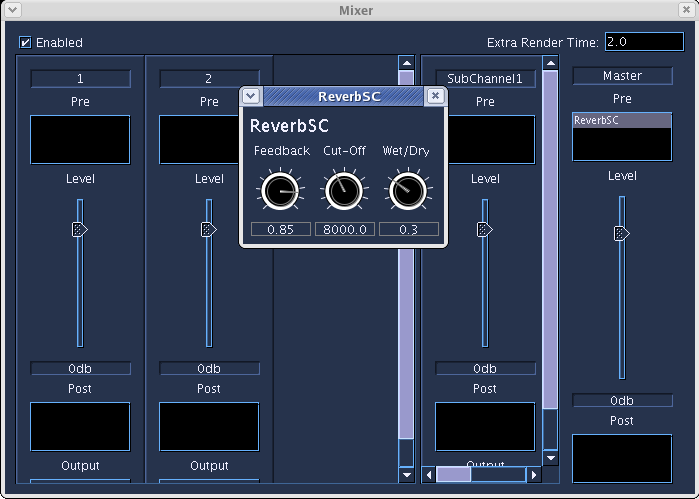
\includegraphics{images/mixer.png}

The Mixer system in blue allows for graphically editing levels for
instruments, applying pre- and post-fader effects, and routing and
mixing of signals through subchannels.


\subsubsection{Architecture}

The Mixer system has three panel sections:

\begin{description}
\item[Channels]
Channels are auto-created and bound to Instrument ID's in the Orchestra
for a Project. In the Mixer Dialog they are located in the first section
on the left within a splitpane that separates them from the SubChannels.
Channels can be set to route to either SubChannels or directly to the
Master Channel.
\item[SubChannels]
SubChannels are user-created and are located in the center section of
the Mixer Dialog, on the right side of the splitpane. Channels can be
set to route to SubChannels, and SubChannels can route into other
SubChannels or out to the Master Channel.
\item[Master Channel]
The Master Channel is located on the right side of the Mixer Dialog.
There is only one master Channel per project which all channel and
subchannel signals ultimately route through.
\end{description}

Each channel allows for applying effects to the incoming signal either
pre- or post-fader.

\subsubsection{Using the Mixer}

For most MIDI-based music composition environments, the typical user
interaction with a Mixer system is that users first create tracks on a
timeline, and for each track an audio channel is automatically bound in
the mixer. The user then selects an instrument for that track(if it is a
MIDI track); MIDI information from the track is routed to the instrument
and that instrument generates audio signals. If the instrument happens
to be a software synthesizer, the audio signals are then usually taken
from the instrument and routed out to the Mixer channel that has been
bound to that track.

However, since blue does not bind music information on a SoundLayer to
an instrument (you can have heterogenous note data generated in any
soundObject for any number of instruments, a flexibility which allows
for soundObjects to be more representative of musical ideas), and nor
does it bind SoundLayers to channels, the abstraction of the musical
system and the interaction with the Mixer system requires different
handling.

In blue's Mixer system, Mixer channels are automatically bound to
instruments by their instrument ID. Binding to ID and not per-instrument
in the Orchestra allows for the case where users have set multiple
instruments to the same instrument ID but only having one which is
enabled. If you then disable one and then enable another instrument to
test out different instruments with the same musical note data, the
mixer channel's settings will be maintained for the new instrument as it
is bound by ID.

Channels in themselves can not be created or removed directly by the
user, but are automatically added or removed depending on how how
instruments are added and removed from the project's orchestra. For
cases of when an instrument has an ID and a user wishes to change the
ID, if the new ID already exists and a channel is already created, the
old channel is removed as long as no other instrument has the old ID. If
the new channel ID has no existing mixer channel bound to it and if the
channel for the old ID only has one instrument with that ID (the
instrument that is changing ID's), the bound mixer channel is simply
reassigned to the new ID and maintains its settings.

Subchannels are added by right-clicking with in the SubChannels area and
choosing "Add SubChannel" from the popup menu. To remove a subchannel
right-click the channel strip to be removed and select "Remove" from the
popup menu.

At the bottom of every Channel and SubChannel strip is an output
dropdown box to choose where to route that Chanel's audio to. For
SubChannels, they can only route to other SubChannels which lead to the
Master Channel, meaning that there is no feedback allowed (i.e. routing
SubChannelA to SubChannelB and then to SubChannelC and that back to
SubChannelA is not allowed as it would create a loop).

For the instruments in the orchestra to be able to route out to the
Mixer, a special pseudo-opcode must be used for the output of the
instrument, entitled "blueMixerOut". You use blueMixerOut in the same
way as the outc opcode. If the Mixer is not enabled in the Dialog, when
blue goes to process the instrument, blueMixerOut will be replaced with
outc, thus making the audio of that instrument directly route out to dac
or disk, depending on how Csound is set to render. If the Mixer is
enabled, blueMixerOut is translated into global variables and the
Mixer's instrument code is generated automatically without the user
having to worry about the code details of setting up a Mixer system
themselves in Csound code.

There is also a subChannel form of blueMixerOut available that is able
to target a subchannel by name. This form is used in the following way:

\begin{verbatim}
      blueMixerOut "subChannelName", asig1, asig2 [, asig3...]
    
\end{verbatim}

Using this form, the asig signals will be mixed into the subChannel
given by name. This form is available to use within Instruments but is
also very useful to use when working Sound SoundObjects and AudioFile
SoundObjects, which do not have channels created for them. This way, you
can route the output of an AudioFile to a named subchannel and apply
Effects, etc.

\subsubsection{Effects}

Effects in blue are implemented as User-Defined Opcodes, and
understanding of how User-Defined Opcodes work in Csound is recommended
before creating Effects. Understanding how UDO's work however is not
necessary if one simply wants to use Effects.

The workflow for using Effects with your Mixer channels is:

\begin{enumerate}
\def\labelenumi{\arabic{enumi}.}
\item
  Populate your Effects Library by either creating effects or importing
  them from blueShare.
\item
  In the Mixer, choose either the pre-fader or post-fader effects bin to
  add effects. Right click on the bins to open up a popup menu that
  shows effects that are currently in your library from which to choose
  to insert.
\item
  In the Mixer, choose either the pre-fader or post-fader effects bin to
  add effects. Right click on the bins to open up a popup menu that
  shows effects that are currently in your library from which to choose
  to insert.
\item
  Configure your effect by double-clicking it in the effects bin.
  Double-clicking the effect will open up a dialog that shows the
  effect's graphical user interface.
\end{enumerate}

Effects Library

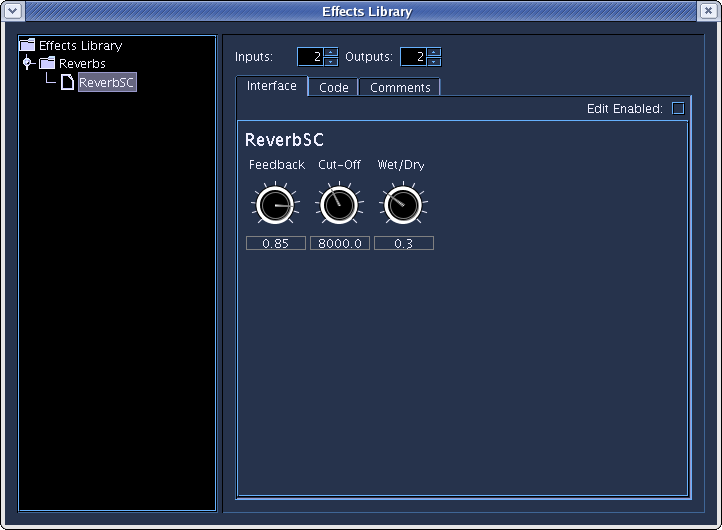
\includegraphics{images/effectsLibrary1.png}

Effects are created and managed in your Effects Library, which is
accessible from the Tools menu. The Effects Library is program wide, so
any Effect in the library will be accessible to use from any project you
are working on.

In the picture above, you will see the library where one can create
Effects as well as organize them into groups. The organization into
groups within the library will be reflected in the Effects popup that
appears when the user is looking to add Effects to their Mixer channels.

To add a group or new Effect, right click on any node and choose the
option from the popup. The popup will also allow you to cut/copy/paste
groups or Effects which is useful when reorganizing or when creating new
Effects based on older ones.

Once an Effect or group is added, you can edit the the name by
double-clicking the node in the tree. Selecting an effect by clicking it
once will populate the editor on the right. The picture above shows the
User Interface editor for the Effect. Like other BlueSynthBuilder-based
editors in blue, clicking Edit Enabled will allow you to move between to
edit modes, one in which you can add, remove, and move around widgets,
and another where you can interact with the widgets (useful for setting
an initial value for the Effect.)

Effects Library

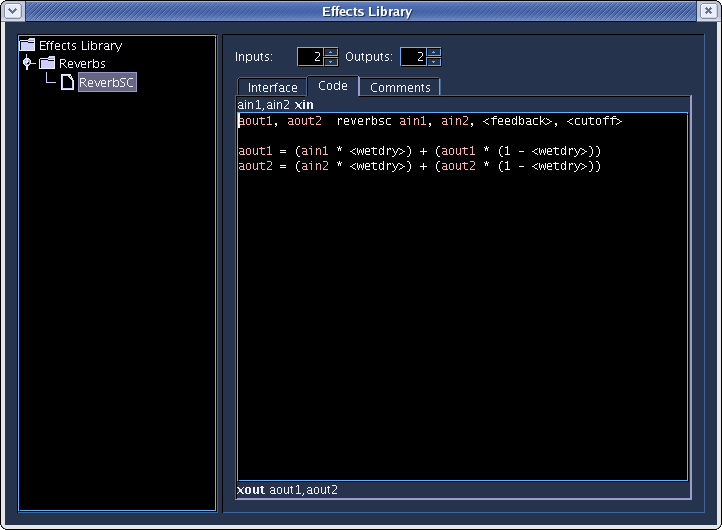
\includegraphics{images/effectsLibrary2.png}

In the code editor for the Effect, one sees that the xin and xout lines
of the User-Defined opcode display according the number of in and out
audio signals the Effect will support. The names of the signals are
hard-coded, which makes it easier for others to know exactly what the
incoming and outgoing signals will be should they look at your code.

Code for the Effect should follow the same principles as User-Defined
Opcodes(i.e. one can add a setksmps line at the top of the code area).
Values from the widgets follow the same principles as BlueSynthBuilder,
and code completion for opcodes (ctrl-space) and BSB widgets
(ctrl-shift-space) work within the code editor.

\begin{quote}
\textbf{Note}

blue currently expects Effects to have nchnls number of channels in and
out where nchnls is the number set by the project.
\end{quote}

\subsubsection{Other Notes}

\begin{itemize}
\item
  The Extra Render Time option in the Mixer dialog allows the user to
  add extra time to the end of the score. This is useful to allow time
  for Effects which may have time delay (i.e. 3-second long reverb) to
  have time enough for processing, as well as simply to add time at the
  end of a piece.
\end{itemize}

\subsubsection{Sends}

Besides effects, users are also able to put in Sends into the pre- and
post-fader Effects bins. Sends will output the signal from that point in
the channel's signal chain to a selected SubChannel. As with the output
channels, Sends can only feed-forward down the chain to the Master Out
and can not be made to create a feedback loop. Users are able to set the
channel to send to as well as the amount to send. This send amount is
also able to be Automated, just as the Effects are.

\subsubsection{Randomization}

Widget values are able to be randomized in the same way as in the
BlueSynthBuilder, and is available in the usage mode when working with
Effects in the Effects Library or when using Effects from the mixer.
Please further information, please see the documentation for
\protect\hyperlink{bsbWidgetRandomization}{BlueSynthBuilder Widget
Randomization}.

\subsubsection{Code Generation Optimization}

blue's mixer system optimizes when generated code for Csound to use.
When compiling down to ORC code, blue checks all signal paths to see if
any path will result in unused audio and if so, will optimize out any
code that is along that path. The rules for optimization are as follows:

\begin{itemize}
\item
  If channel does not generate signal to channel output (if no
  automation for level fader and fader == -96.0f), only generate code up
  to last send in preFader effects chain
\item
  When processing Sends, checks down the graph to see if send signal
  will make it to the Master output or not, checking both down graph of
  output channels as well as sends for each channel. If not, does not
  generate output for Send.
\item
  If channel does not have channel output and no valid prefader sends,
  do not generate anything for channel.
\item
  If SubChannel has no signal inputs (whether it's from another
  Channel's out channel, a Send, or dependency from code that uses the
  subChannel form of blueMixerOut), do not generate anything for
  channel.
\end{itemize}

\subsection{Blue Live}\label{blueLive}

Blue Live

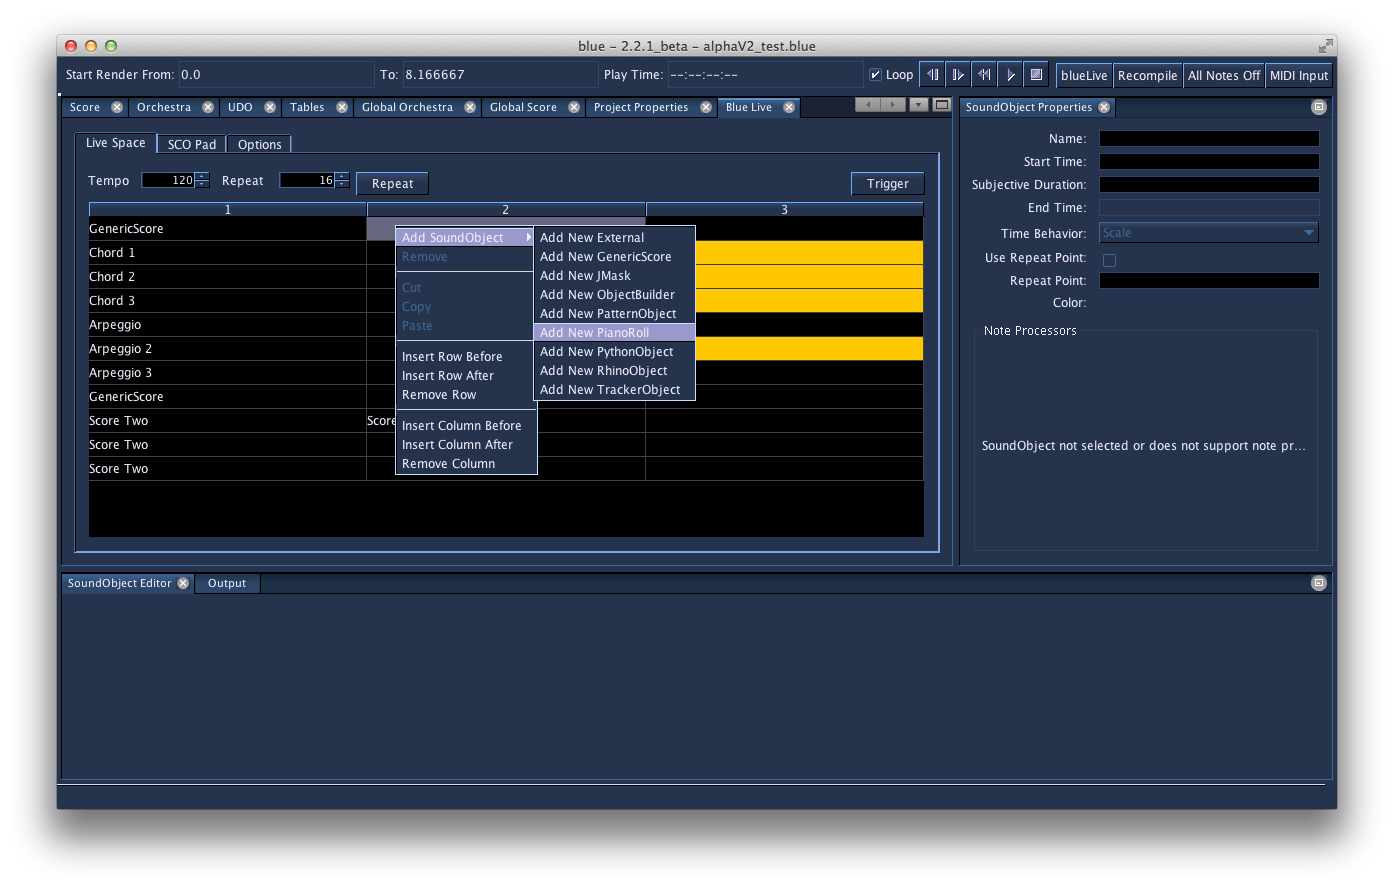
\includegraphics[width=1.00000\textwidth]{images/blueLive.png}

Blue Live allows you to work with Csound in realtime. It allows for
generating score with SoundObjects and working with MIDI keyboard input
to create notes and run with Csound instruments defined in your project.
Note: Blue Live works when using the Csound API, or on non-Windows
platforms when not using the Csound API. Windows does not allow piping
text to executable in a non-blocking way and therefore limits what can
be done when not using the API.

\subsubsection{Motivation}

The motivation of Blue Live is primarily to aid the composer in working
out ideas and to help configure instrument, effects, and mixer settings.
You may find it helpful early on within the life a composition, when you
want to try out a number of different ideas in realtime. You may tweak
instrument parameters, mixer settings, try out different notes and
chords with a MIDI keyboard, and even work with different SoundObjects.
Later, when you have some ideas worked out, you can take your
SoundObjects from blueLive into your score timeline and continue working
from there.

Beyond this primary capacity as a mode to aid composition, Blue Live has
some capacity to be used for realtime performance. The focus of Blue
Live's development is as a compositional aid first, and performance
second, though work continues to expand its usefulness in both regards.

\subsubsection{Working with Blue Live}

Blue Live is designed to work with the rest of your blue project file.
When Blue Live is turned on, the blue project generates everything from
the project except for the Score generated from the Score timeline. The
Global Score text will be used, but instead of
\textless{}TOTAL\_DUR\textgreater{} being calculated from the score
timeline, a default value of 3600 is used. This allows your notes that
would be used for effects instruments to run for 3600 seconds (this size
can be modified; please make a request if desired).

The main toolbar has four buttons for blue Live:

\begin{description}
\item[blueLive]
Toggle button that stops and starts blueLive
\item[Recompile]
If blueLive is running, this button will cause blue to recompile the CSD
from your project and restart blueLive. This is useful if you modify
your orchestra code and want to quickly recompile and continue working
with blueLive.
\item[All Notes Off]
Turns off any score notes that are actively playing
\item[MIDI Input]
Toggle button that turns on and off the configured MIDI devices setup in
Program Options (discussed further below).
\end{description}

The primary Blue Live window is available from the Window Menu, or by
using the ctrl-8 shortcut. The Blue Live window has three main tabs: the
Live Space, the SCO Pad, and Options. These will be discussed int he
following sections.

\subsubsection{Live Space}

The Live Space is an area to work with SoundObjects. It is a table
divided into bins and rows of spaces to place SoundObjects. SoundObjects
can be copied to/from the Score Timeline as well as the Live Space.
SoundObjects can also be created within the Live Space by right clicking
an empty bin within the bins and choosing "Add SoundObject" from the
popup menu. Clicking on an occupied bin will select that SoundObject.
The properties for the SoundObject can be modified using the SoundObject
Properties Window, and the contents of the SoundObject can be modified
from the SoundObject Editor Window. Besides the selected and unselected
states, you can double-click a soundObject to put it into an enabled
state. Enabled objects are highlighted in orange and are the
SoundObjects that are triggered when multi-trigger or repeat is used.

Once a SoundObject is added to the Live Space, it can be triggered in
one of two ways:

\begin{description}
\item[Single Trigger]
Trigger the contents of the currently selected SoundObject. This is done
by using the keyboard shortcut ctrl-T (cmd-T on OSX).
\item[Multi Trigger]
Triggers the contents of the currently enabled SoundObjects. This is
done either by using the Trigger button, or using the keyboard shortcut
ctrl-shift-T (cmd-shift-T on OSX).
\end{description}

Triggering a soundObject will take the score generated from it and pass
it immediately to the active Csound instance for blueLive (blueLive must
be running for this to work). Scores are always generated with Time
Behavior of None, processed through their NoteProcessors, then scaled
according to the given tempo.

One can turn on Repeat to cause repeated trigger of enabled SoundObjects
according to the tempo given and the number of beats in which to
retrigger. For example, using a repeat of 4 means it will re-trigger
every four beats. The score is processed as mentioned above, but there
is no truncation done. Therefore, if a SoundObject generates a score of
8 beats, and there is a repeat of 4 beats, when the repeat occurs, there
will be 4 beats of overlap between the first trigger and the second
trigger.

When Repeat is on, it will always finish out the current number of beats
in the repeat at the current tempo, before applying any changes to tempo
and repeat. Modifyications to tempo and repeat will apply then on the
next repeat trigger.

\subsubsection{SCO Pad}

\begin{quote}
\textbf{Note}

This feature will likely be removed in a future release.
\end{quote}

This is an experimental feature to record MIDI input in a manner similar
to to notation programs (press keys, then press 4 for a quarter note, 8
for and 8th note, etc.). This feature requires MIDI Input to be turned
on. This feature is experimental at this time.

\subsubsection{Options}

The options panel allows setting up parameters for blue Live. Currently
it contains options for modifying the commandline string used when
running blueLive. For most users, these modification will not be
necessary and the default commandline used will be sufficient.

\subsubsection{Working with MIDI}

blue's MIDI system, when enabled, will listen to configured MIDI devices
for notes, map the key and velocity, and generate Csound notes to
achieve MIDI-like note-on and note-off type behavior. This allows
working with a MIDI keyboard in realtime with your project instruments
without modifying your instruments specifically for MIDI. This also
means that when blue's MIDI system is enabled, Csound MIDI processing
should be disabled for your project.

To configure what MIDI devices to use, go to the program Options
settings (on OSX it is the application's Preferences, on other platofrms
it is the Options menu item in the Tools menu) and under "blue", go to
MIDI. There you will see a list of MIDI devices connected to your
computer. If you connected a device after starting blue, you can rescan
to find your MIDI device. In this window you will configure what MIDI
devices you want to use with blue, but these devices will not be opened
for listening until you enable MIDI Input on the blueLive toolbar in the
main application.

Once you have configured what devices to use with blue, return to the
main program and enable MIDI input using the "MIDI Input" button, then
start blueLive. At this point, when MIDI notes are played, blue will
take the incoming note data, map it according to the values configured
in the MIDI Input Panel window (available from the Windows Menu), and
then generate notes and pass them to Csound.

For a MIDI note on, blue will the channel number of the note and map it
to the instrument in the orchestra manager by index. For example, if you
have three instruments numbered 1, 3, and 5, notes for MIDI channel 1
will generate with instr 1, notes for MIDI channel 2 will generate with
instr 3, and notes for MIDI channel 3 will generate with instr 5.

The MIDI key number as well as the velocity will be mapped according to
the settings set in the MIDI Input Panel window. This allows for
generating frequency, Csound PCH, and using Scala Tuning files to
generate either frequencies or bluePCH format text, amongst other
values.

Instruments that are intended to be used with blue's MIDI system will
have to work with a 5 p-field note format. This does not mean your
instrument can only work with 5 p-fields, but rather that your
instrument must support at least that. An example blue project can be
found in examples/features/blueLiveMidi.blue (if you are using the OSX
application, you may need to explore the contents of the blue.app
program to find the examples folder).

\subsubsection{Exploring Ideas}

Blue Live uses a subset of the same soundObjects that are available on
the score timeline within the main editing window of blue. Some possible
ways you could explore ideas are:

\begin{itemize}
\item
  trying out SCO ideas with genericScore
\item
  testing your python functions with the pythonObject
\item
  testing your javaScript functions with the rhinoObject
\item
  using Cmask, nGen, Common Music, and other programs with the external
  soundObject to try out things live
\end{itemize}

\subsection{Tables Manager}\label{tablesManager}

Tables Manager

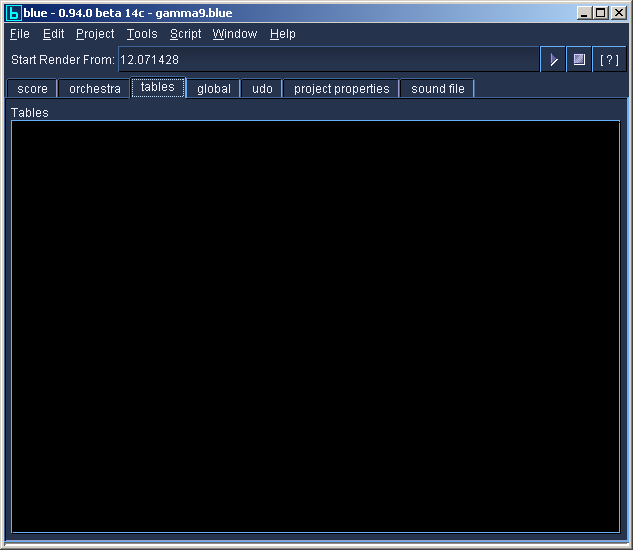
\includegraphics{images/tablesTab.png}

The tables manager contains a text area for global tables. Table
statements put here will be immediately inserted above i-statements of
the \textless{}CsScore\textgreater{} area of the generated CSD file.

\subsection{Globals Manager}\label{globalsManager}

Csound Orchestra and Score text can be passed directly into a generated
CSD by using the Global Orchestra and Global Score windows.

Anything here will be inserted into the
\textless{}CsOrchestra\textgreater{} section of the .CSD file before
anything generated by the Orchestra. Things like global variables,
macros, or GUI instrument definitions may go here.

Anything here will be inserted into \textless{}CsScore\textgreater{}
section of the .CSD file before anything generated by the score
timeline. the global score's processing is done outside of the score
timelines, so any notes put here are not factored into values calculated
from the timeline, like total duration, nor are any notes in the global
score section translated like the timeline is when a different start
time is used other than 0.0. for instance, if you use 2.0 as a start
time, a note in the score timeline at 2.0 will be translated to start at
0.0, while a note with a start time of 2.0 in the global score section
is not affected and will start at time 2.0.

There are also certain variables made available from blue (blue
variables) that are useful for specific purposes. One of them is
\textless{}TOTAL\_DUR\textgreater{}. An example of its use is:

\begin{verbatim}
i20 0 [<TOTAL_DUR> + 10] .95 1 1000
\end{verbatim}

The note given above is for a global effect(a global reverb unit). This
note will always start at time zero regardless of when the score starts,
and will always last as long as the duration of the generated score from
the timeline plus 10 seconds. Because blue variables are a text swap,
the above use of the bracket notation that Csound uses was necessary.
For a score with a 20 second duration, the above note would have been
generated as:

\begin{verbatim}
i20 0 [20 + 10] .95 1 1000
\end{verbatim}

Because of the blue variable used, the note will correclty play
regardless of when the score starts. If the the blue variable was note
used and was put as a note in the Score timeline, the reverb may not
run.

\begin{quote}
\textbf{Note}

When blue variables were created, blue did not have a Mixer system
implemented. The above system continues to function, the practice of
using the Mixer is highly recommended. This feature is left in for
legacy projects.
\end{quote}
